% !TEX program = lualatex
\documentclass[a4paper,12pt]{extarticle}
\usepackage{amsmath}
\usepackage{hyperref}
\hypersetup{
    colorlinks=true,    % Enables colored links
    linkcolor=blue,     % Color for internal links (e.g., table of contents)
    citecolor=blue,     % Color for citations
    filecolor=blue,     % Color for file links
    urlcolor=blue       % Color for URLs
}
\usepackage{fontspec}

\usepackage{polyglossia}
\setdefaultlanguage{ukrainian}

% Встановлюємо Times New Roman як основний шрифт
\setmainfont{Times New Roman}
\newfontfamily\cyrillicfont{Times New Roman}
\newfontfamily\cyrillicfonttt{JetBrainsMono Nerd Font}

\usepackage{geometry}
\geometry{top=25mm,bottom=15mm,left=25mm,right=10mm} % Встановлення полів сторінки

\usepackage{titlesec}
\titleformat{\section}{\normalfont\large\bfseries\centering}{}{0pt}{}
\titleformat{\subsection}{\normalfont\bfseries\centering}{}{0pt}{}
\titleformat{\subsubsection}{\normalfont\bfseries\itshape}{}{0pt}{}

\setlength{\parindent}{12.5mm}  % Встановлення загального абзацного відступу
\newcommand{\address}{\hspace*{90mm}} % Відступ для адресата
\newcommand{\approval}{\hspace*{100mm}} % Відступ для «Гриф затвердження»
\newcommand{\signature}{\hspace*{125mm}} % Відступ для підпису

\usepackage{setspace}

\pagenumbering{arabic} % Встановлення арабської нумерації

\usepackage{amsmath} % Для розширених математичних виразів
\usepackage{amsthm} % Для середовища доказів

\usepackage{enumitem}
\setlist[enumerate,2]{label=\theenumi.\arabic*} % Нумерація = попередній.наступний рівень
\setlist[enumerate,3]{label=\theenumii.\arabic*} % Нумерація = попередній.попередній.наступний рівень

\usepackage{svg} % Для вставки блок-схем у форматі SVG
\usepackage{float} % Для керування розміщенням блок-схем

% Встановлюємо шрифт JebBrainsMono Nerd Font як моноширинний
\setmonofont{JetBrainsMono Nerd Font}

% Визначення кольорів, натхнених темою Solarized Light
\definecolor{background}{HTML}{FFFFFF} % Світлий кремовий
\definecolor{keyword}{HTML}{268BD2}    % М'який синій
\definecolor{string}{HTML}{2AA198}     % Бірюзовий
\definecolor{comment}{HTML}{93A1A1}    % Сірий
\definecolor{function}{HTML}{859900}   % Оливковий зелений
\definecolor{variable}{HTML}{B58900}   % Гірчичний жовтий
\definecolor{type}{HTML}{D33682}       % Пурпуровий

\usepackage{listings}       % Для підсвітки синтаксису
\usepackage{xcolor}       % Для роботи з кольорами

% Налаштування listings із кастомним шрифтом та кольоровою схемою
\lstset{
	basicstyle=\footnotesize\ttfamily,          % Використання \ttfamily для моноширинного шрифту
	backgroundcolor=\color{background},
	keywordstyle=\color{keyword}\bfseries,
	stringstyle=\color{string},
	commentstyle=\color{comment}\itshape,
	identifierstyle=\color{variable},
	emphstyle={\color{function}},
	numberstyle=\tiny\color{comment},
	numbers=left,
	numbersep=5pt,
	tabsize=4,
	frame=lines,
	breaklines=true,
	xleftmargin=10pt,    % Опційно: корекція лівого відступу
	xrightmargin=10pt,   % Опційно: корекція правого відступу
	% Налаштування ширини символів (зменшити при потребі)
	columns=fullflexible  % Дозволити більшу гнучкість у ширині символів
}

\usepackage{multicol}
\usepackage{pgffor}


\newcommand{\labnumber}{6}
\newcommand{\labtopic}{Використання динамічних масивів.}
\newcommand{\labtask}{Написати програму розв'язання системи лінійних алгебраїчних рівнянь (СЛАР) методом простої ітерації з використанням динамічних масивів}
\newcommand{\labdate}{«13» грудня 2024 р.}

\newcommand{\includelistings}[2]{%
	\foreach \filename in {#1} {%
		\subsubsection{\filename}%
		\lstinputlisting[language=#2]{\filename}%
	}%
}

\begin{document}

\doublespacing
\begin{titlepage}
	\begin{center}
		{\fontsize{14pt}{16pt}\selectfont\textbf{КПІ ім. Ігоря Сікорського} \\
			\textbf{Факультет інформатики та обчислювальної техніки} \\
			\textbf{Кафедра інформатики та програмної інженерії}}\\
	\end{center}

	\vspace{1cm}

	\begin{center}
		{\fontsize{14}{16pt}\selectfont\textbf{Звіт до комп'ютерного практикуму з курсу}\\
			\textbf{«Основи програмування»}\\}
	\end{center}

	\vspace{6cm}

	\singlespacing
	\begin{multicols}{3}
		{
			\raggedright
			\fontsize{12pt}{12pt} \selectfont
			Прийняв \\
			асистент кафедри ІПІ \\
			Ахаладзе А. Е. \\
			\labdate
		}

		\columnbreak
		\vfill\null
		\columnbreak

		{
			\raggedright
			\fontsize{12pt}{14pt} \selectfont
			Виконав \\
			студент групи ІП-43 \\
			Дутов І. А. \\
		}
	\end{multicols}

	\vfill
	\begin{center}
		{\fontsize{14}{16}\selectfont\textbf{Київ 2024}}
	\end{center}
\end{titlepage}
\newpage

\singlespacing

\section{Комп'ютерний практикум №\labnumber}
\vspace{-10pt}
\begin{center}
	\emph{\textbf{Тема:} \labtopic}
\end{center}
\vspace{-5pt}

\textbf{Завдання:}\\
\indent \labtask.

\subsection{Текст програми}
\includelistings{../src/main.c, ../src/common/constants.h, ../src/common/types.h, ../src/algorithm.h, ../src/algorithm.c, ../src/io/equations.c, ../src/io/equations.h, ../src/io/utils.h, ../src/io/utils.c, ../src/io/int.h, ../src/io/int.c, ../src/io/double.h, ../src/io/double.c, ../src/io/validators.h, ../src/io/validators.c}{C}
\includelistings{../meson.build}{bash}

\subsection{Введені та одержані результати}

\newgeometry{left=0mm, right=0mm}
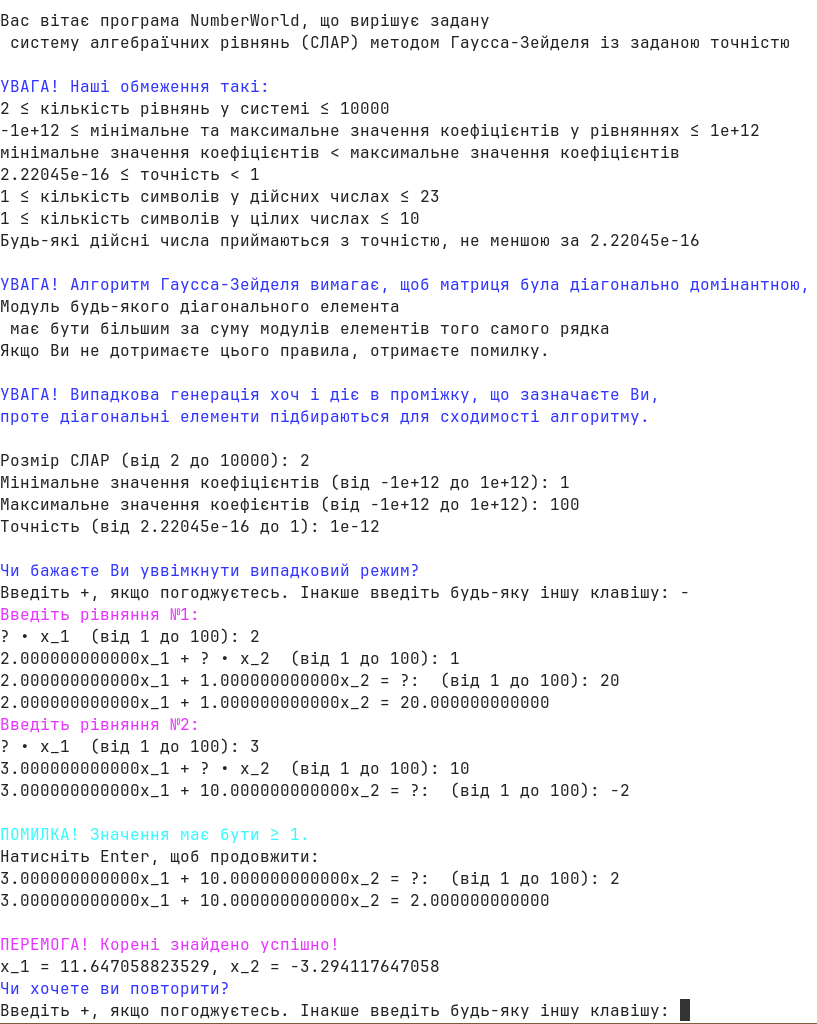
\includegraphics[height=\textheight]{examples/example1.png}\\
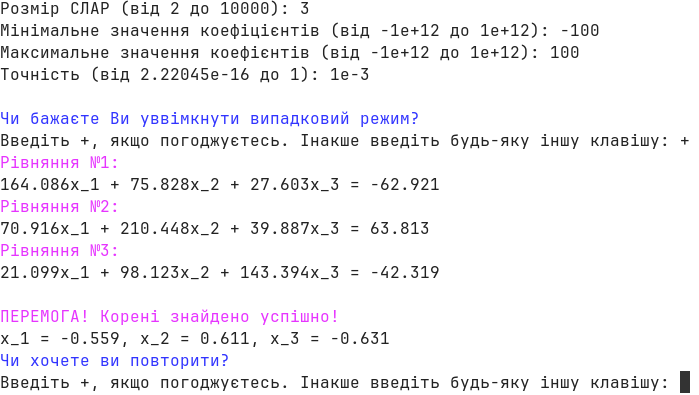
\includegraphics[width=\textwidth]{examples/example2.png}\\
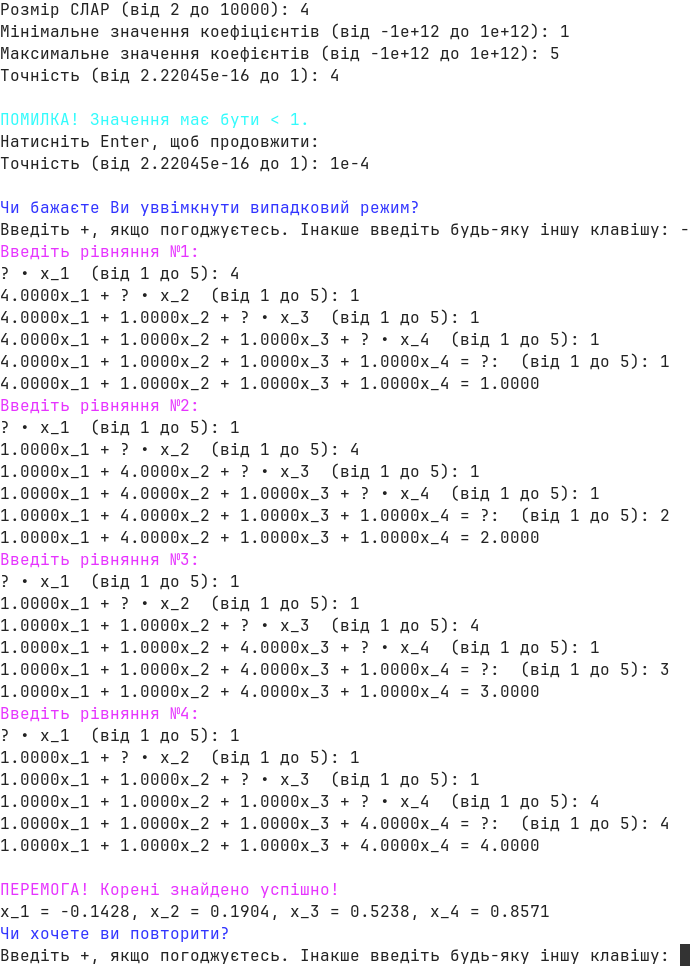
\includegraphics[height=\textheight]{examples/example3.png}\\
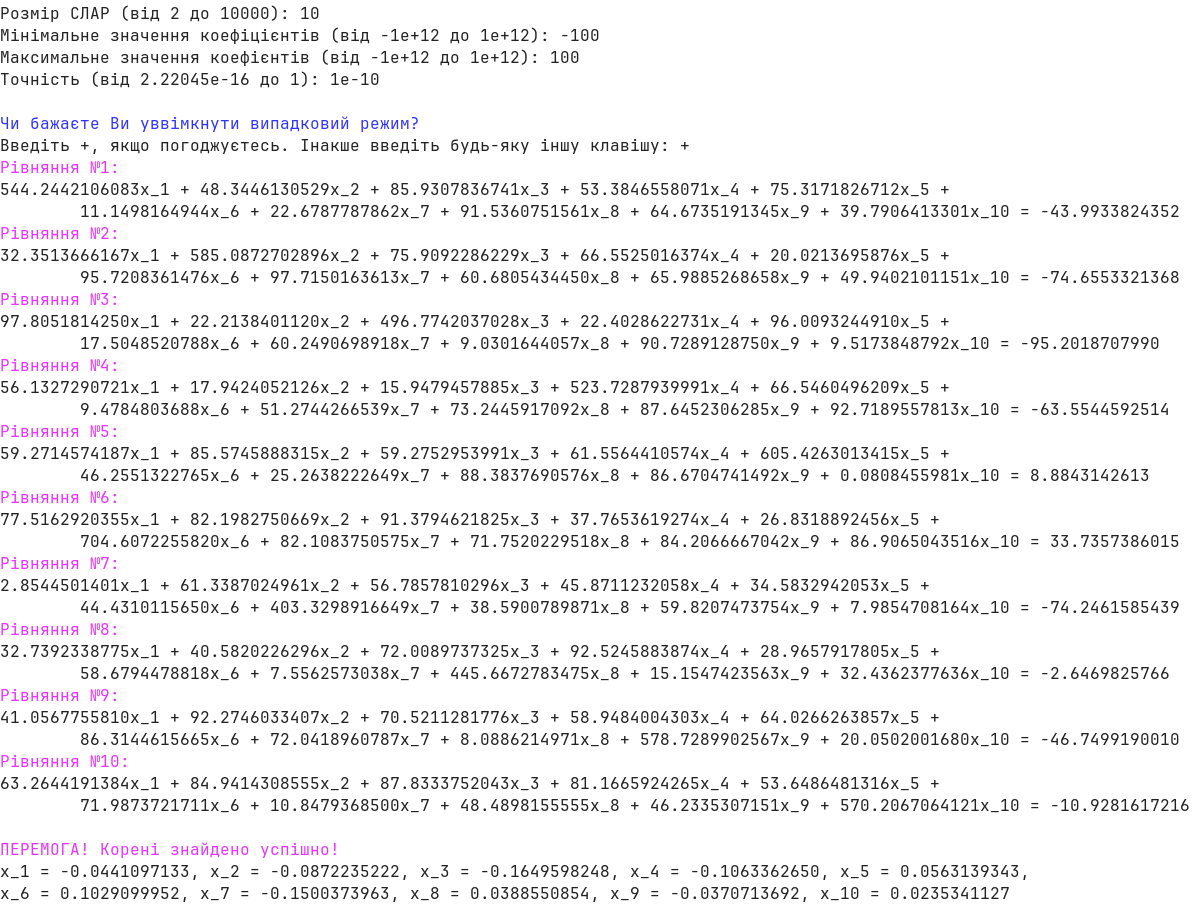
\includegraphics[width=\textwidth]{examples/example4.png}
\restoregeometry

\subsection{Теоретичні розрахунки}
Слід виконати перевірку відповідей підстановкою коренів у рівняння:

\textbf{Випадок 1.}
\newcommand{\x}{11.647058823529}
\newcommand{\y}{-3.294117647058}

$2 \cdot \x + 1 \cdot \y = 20$ == 20 \\
$3 \cdot \x + 10 \cdot \y = 2.0000000000069917$ \approx 2

\textbf{Випадок 2.}
\renewcommand{\x}{-0.559}
\renewcommand{\y}{0.611}
\newcommand{\z}{-0.631}

$164.086 \cdot \x + 75.828 \cdot \y + 27.603 \cdot \z = -62.810659000000015 \approx$ -62.921 \\
$70.916 \cdot \x + 210.448 \cdot \y + 39.887 \cdot \z = 63.77298700000001 \approx$ 63.813 \\
$21.099 \cdot \x + 98.123 \cdot \y + 143.394 \cdot \z = -42.32280200000001 \approx$ -42.319

\textbf{Випадок 3.}
\renewcommand{\x}{-0.1428}
\renewcommand{\y}{0.1904}
\renewcommand{\z}{0.5238}
\newcommand{\w}{0.8571}

$4 \cdot \x + 1 \cdot \y + 1 \cdot \z + 1 \cdot \w = 1.0001 \approx$ 1 \\
$1 \cdot \x + 4 \cdot \y + 1 \cdot \z + 1 \cdot \w = 1.9997 \approx$ 2 \\
$1 \cdot \x + 1 \cdot \y + 4 \cdot \z + 1 \cdot \w = 2.9999000000000002 \approx$ 3 \\
$1 \cdot \x + 1 \cdot \y + 1 \cdot \z + 4 \cdot \w = 3.9998 \approx$ 4

\textbf{Випадок 4.}
\href{https://matrixcalc.org/slu.html#solve-using-Gaussian-elimination%28%7B%7B5442442106083,397906413301,483446130529,859307836741,533846558071,753171826712,111498164944,226787787862,915360751561,646735191345,-439933824352%7D,%7B323513666167,499402101151,5850872702896,759092286229,665525016374,200213695876,957208361476,977150163613,606805434450,659885268658,-746553321368%7D,%7B978051814250,95173848792,222138401120,4967742037028,224028622731,960093244910,175048520788,602490698918,90301644057,907289128750,-952018707990%7D,%7B561327290721,927189557813,179424052126,159479457885,5237287939991,665460496209,94784803688,512744266539,732445917092,876452306285,-635544592514%7D,%7B592714574187,808455981,855745888315,592752953991,615564410574,6054263013415,462551322765,252638222649,883837690576,866704741492,88843142613%7D,%7B775162920355,869065043516,821982750669,913794621825,377653619274,268318892456,7046072255820,821083750575,717520229518,842066667042,337357386015%7D,%7B28544501401,79854708164,613387024961,567857810296,458711232058,345832942053,444310115650,4033298916649,385900789871,598207473754,-742461585439%7D,%7B327392338775,324362377636,405820226296,720089737325,925245883874,289657917805,586794478818,75562573038,4456672783475,151547423563,-26469825766%7D,%7B410567755810,200502001680,922746033407,705211281776,589484004303,640266263857,863144615665,720418960787,80886214971,5787289902567,-467499190010%7D,%7B632644191384,5702067064121,849414308555,878333752043,811665924265,536486481316,719873721711,108479368500,484898155555,462335307151,-109281617216%7D%7D%29}{Розв'язки цілком співпадають зі знайденими коренями.}\\
\begin{center}
	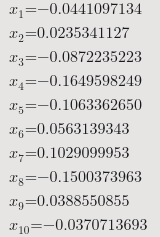
\includegraphics{examples/visual.png}\\
\end{center}
\emph{\textbf{Висновки:}} Програма працює коректно. Програма вирішує поставлене завдання.

\end{document}
